\documentclass[aspectratio=169]{beamer}

%%%%%% 导入包 %%%%%%
\usepackage{xeCJK}
\usepackage{graphicx}
\usepackage{xcolor}
\usepackage{cite}
\usepackage{indentfirst}
\usepackage{amsmath}
\usepackage{amssymb}
\usepackage{times}

\usepackage{ctex}
\usepackage{geometry}
\usepackage{graphicx}
\usepackage{multirow}
\usepackage{array}
\usepackage{float}

\usepackage[super,square,comma,sort&compress]{natbib}
\usepackage{listings}
\usepackage{xcolor}
\colorlet{punct}{red!60!black}
\definecolor{background}{HTML}{EEEEEE}
\definecolor{delim}{RGB}{20,105,176}
\colorlet{numb}{magenta!60!black}

\lstdefinelanguage{json}{
    basicstyle=\ttfamily\scriptsize,
    numbers=left,
    numberstyle=\ttfamily\scriptsize,
    stepnumber=1,
    numbersep=4pt,
    showstringspaces=false,
    breaklines=true,
    frame=lines,
    % backgroundcolor=\color{background},
    literate=
     *{0}{{{\color{numb}0}}}{1}
      {1}{{{\color{numb}1}}}{1}
      {2}{{{\color{numb}2}}}{1}
      {3}{{{\color{numb}3}}}{1}
      {4}{{{\color{numb}4}}}{1}
      {5}{{{\color{numb}5}}}{1}
      {6}{{{\color{numb}6}}}{1}
      {7}{{{\color{numb}7}}}{1}
      {8}{{{\color{numb}8}}}{1}
      {9}{{{\color{numb}9}}}{1}
      {:}{{{\color{punct}{:}}}}{1}
      {,}{{{\color{punct}{,}}}}{1}
      {\{}{{{\color{delim}{\{}}}}{1}
      {\}}{{{\color{delim}{\}}}}}{1}
      {[}{{{\color{delim}{[}}}}{1}
      {]}{{{\color{delim}{]}}}}{1},
}


\lstset{
    columns=flexible,
    tabsize = 4,
    basicstyle=\ttfamily\scriptsize,                     % 字体大小
    backgroundcolor=\color{white},                       % 背景颜色
    numbers=left,                                        % 在左侧显示行号
    keywordstyle=\color[RGB]{40,40,255},                 % 设定关键字颜色
    % frame=trbl,
    stepnumber=1,
    numbersep=4pt,
    breaklines=true,
    frame=lines,
    numberstyle=\ttfamily\scriptsize\color{darkgray},    % 设定行号格式
    commentstyle=\it\color[RGB]{0,96,96},                % 设置代码注释的格式
    stringstyle=\rmfamily\slshape\color[RGB]{128,0,0},   % 设置字符串格式
    showstringspaces=false,                              % 不显示字符串中的空格
    language=python,                                     % 设置语言
}
\mode<presentation>
{
  \usetheme{CambridgeUS}
  \usecolortheme{beaver}
  \usefonttheme{default}      % or try serif, structurebold, ...
  \setbeamertemplate{navigation symbols}{}
  \setbeamertemplate{caption}[numbered]
}

\usepackage[english]{babel}
\usepackage[utf8x]{inputenc}
\usepackage{graphicx}
\usepackage{ulem}

\setbeamertemplate{itemize items}{\color{black}$\bullet$}
\graphicspath{{Pictures/}}

\defbeamertemplate{subsection in toc}{bullets}{%
  \leavevmode
  \parbox[t]{1em}{\textbullet\hfill}%
  \parbox[t]{\dimexpr\textwidth-1em\relax}{\inserttocsubsection}\par}

\defbeamertemplate{section in toc}{sections numbered roman}{%
  \leavevmode%
  \MakeUppercase{\romannumeral\inserttocsectionnumber}.\ %
  \inserttocsection\par}

\setbeamertemplate{section in toc}[sections numbered roman]
\setbeamertemplate{subsection in toc}[bullets]

%%%%%%%%%%%%%%%%%%%%%%%%%%%%%%%%%%%%%%%%%%%%%%%%%%%%%%%%%%%%%%%%%%%%%%%%%%%%%%%%%%
%%%%%%%%%%%%%                       Title                         %%%%%%%%%%%%%%%%
%%%%%%%%%%%%%%%%%%%%%%%%%%%%%%%%%%%%%%%%%%%%%%%%%%%%%%%%%%%%%%%%%%%%%%%%%%%%%%%%%%
\title[电信提高1501]{面向知乎QAWEB的网络爬虫设计与实现}
\author{游浩然 \\ 黎张帆 \\ 郭金城\\}
\institute[\bf HUST]{u201515429\quad u201514574\quad u201511174\quad @hust.edu.cn}
\medskip
\date{\today}

\begin{document}

\begin{frame}
  \titlepage
\end{frame}

%%%%%%%%%%%%%%%%%%%%%%%%%%%%%%%%%%%%%%%%%%%%%%%%%%%%%%%%%%%%%%%%%%%%%%%%%%%%%%%%%%
%%%%%%%%%%%%%                       Content                       %%%%%%%%%%%%%%%%
%%%%%%%%%%%%%%%%%%%%%%%%%%%%%%%%%%%%%%%%%%%%%%%%%%%%%%%%%%%%%%%%%%%%%%%%%%%%%%%%%%

\AtBeginSection[]
{
\begin{frame}<beamer>{Table of Contents}
\tableofcontents[currentsection,currentsubsection,
    hideothersubsections,
    sectionstyle=show/shaded,
]
\end{frame}
}

%%%%%%%%%%%%%%%%%%%%%%%%%%%%%%%%%%%%%%%%%%%%%%%%%%%%%%%%%%%%%%%%%%%%%%%%%%%%%%%%%%
%%%%%%%%%%%%%                       Section                       %%%%%%%%%%%%%%%%
%%%%%%%%%%%%%%%%%%%%%%%%%%%%%%%%%%%%%%%%%%%%%%%%%%%%%%%%%%%%%%%%%%%%%%%%%%%%%%%%%%

\section{Introduction}
% frame 1
\begin{frame}{项目描述}
\begin{itemize}
  \item 爬虫控制端:启动爬虫,停止爬虫,监视爬虫的运行情况
  \item 爬虫运行模块:包含三个小模块,URL管理器、网页下载器、网页解析器
  \begin{itemize}
    \item URL管理器:对需要爬取的URL和已经爬取过的URL进行管理,可以从其中取出待爬取的URL传递给网页下载器。
    \item 网页下载器:网页下载器将URL指定的网页下载下来,存储成一个字符串,传递给网页解析器。
    \item 网页解析器:网页解析器解析传递的字符串,解析器不仅可以解析出需要爬取的数据,而且还可以解析出每一个网页指向其他网页的URL,这些URL被解析出来会补充进URL管理器。
  \end{itemize}
  \item 数据输出模块:存储爬取的数据
\end{itemize}
\end{frame}

\begin{frame}{开发平台}
\begin{itemize}
  \item 硬件平台:个人PC,可连接WEB网络
  \item 软件环境:
  \begin{itemize}
    \item 操作系统:WINDOWS 10 \& Ubuntu
    \item IDE:PyCharm Community Edition 2017.2.3
    \item Python版本:Python 3.6.3 |Anaconda, Inc.| (default, Oct 15 2017, 03:27:45)
  \end{itemize}
  \item 项目所需库
  \begin{itemize}
    \item Wxpthon: Python GUI库
    \item Selenium: Python 模拟浏览器操作库
    \item Phantom:基于selenium的Python工业化模拟浏览器操作库,需设置运行路径或将bin文件夹放入系统路径中。
  \end{itemize}
\end{itemize}
\end{frame}

\begin{frame}{任务分工}
\begin{table}[!htbp]
  \centering
  \renewcommand\arraystretch{1.5}
 	\resizebox{\textwidth}{!}{
    \begin{tabular}{|c|c|c|c|}
 		\hline
 		\qquad ~~姓名~~~~~  & \qquad ~~负责模块~~~~~ & \qquad ~~主要任务~~~~  \\
 		\hline
        \qquad ~~黎张帆~~~~  & \qquad ~~爬虫控制器~~~ & \qquad ~~启动、停止、监视爬虫的运行情况;实现多线程爬取。GUI设计~~~ \\
        \hline
        \qquad ~~游浩然~~~~  & \qquad ~~爬虫运行模块~~~ & \qquad ~~知乎登陆;URL管理器、网页下载器、网页解析器;动态加载~~~ \\
        \hline
        \qquad ~~郭金城~~~~  & \qquad ~~数据输出模块~~~ & \qquad ~~通过网页标签抓取问题URL下的相关信息;动态加载~~~ \\
        \hline
 	\end{tabular}
    }
 \end{table}
\end{frame}
%%%%%%%%%%%%%%%%

\section{Method}
\subsection{整体框架设计}
\begin{frame}{框架}
\begin{figure}
  \centering
  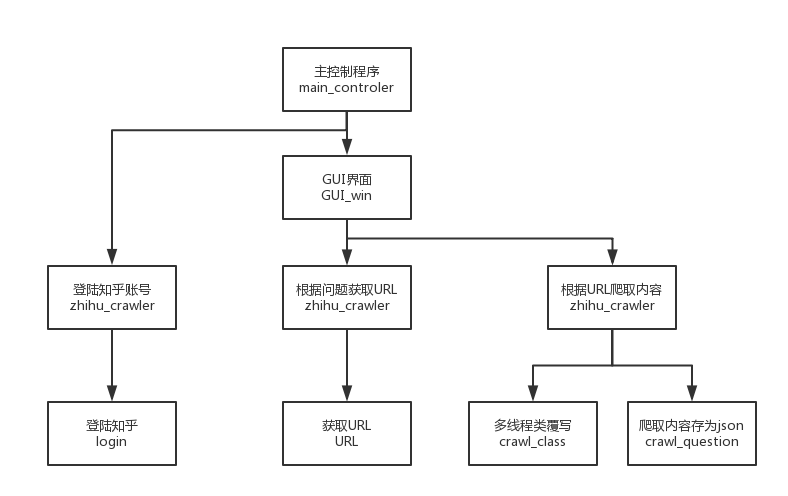
\includegraphics[width=10cm,height=6cm]{模块关系}
  \caption{整体框架设计}
\end{figure}
\end{frame}

\subsection{爬虫控制模块}
\begin{frame}{GUI使用说明}
\begin{columns}
\column{8cm}
\begin{figure}
  \centering
  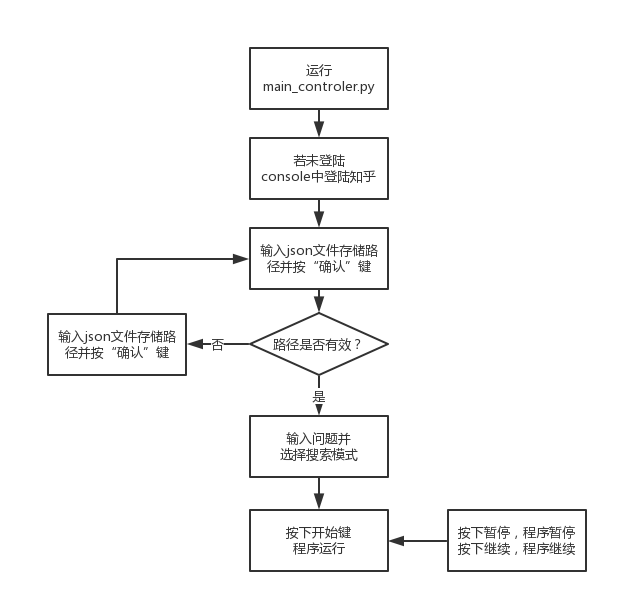
\includegraphics[width=6.5cm,height=5.5cm]{GUI使用说明}
  \caption{GUI使用说明}
\end{figure}

\column{7cm}
\begin{figure}
  \centering
  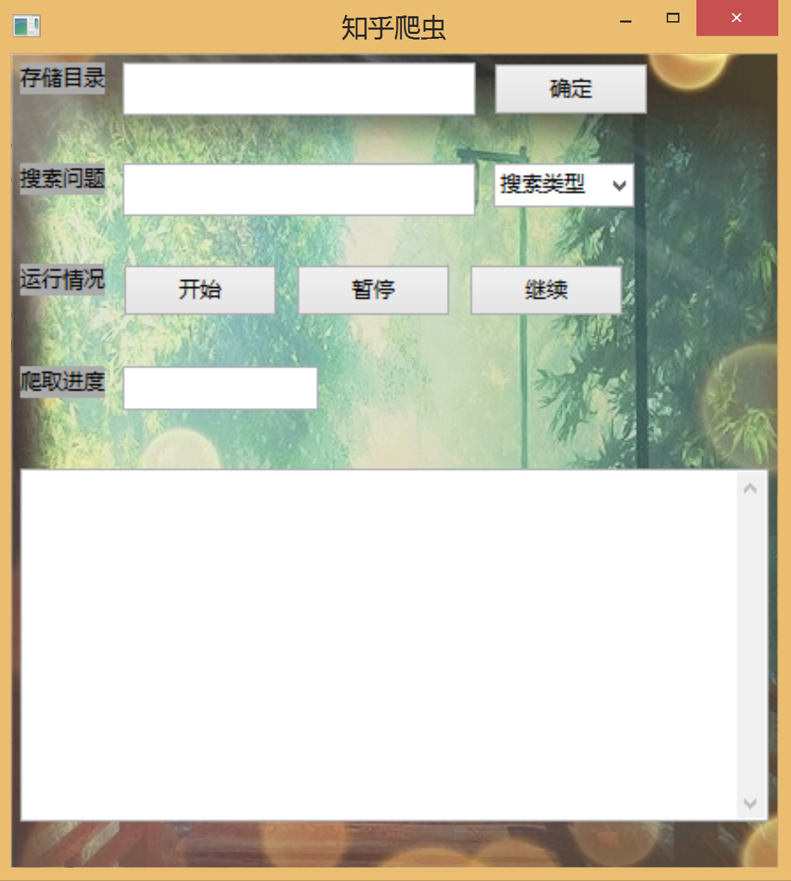
\includegraphics[width=6cm,height=5.5cm]{GUI界面}
  \caption{GUI界面}
\end{figure}
\end{columns}
\end{frame}

\begin{frame}{GUI设计}
\begin{columns}
\column{8cm}
\begin{figure}
  \centering
  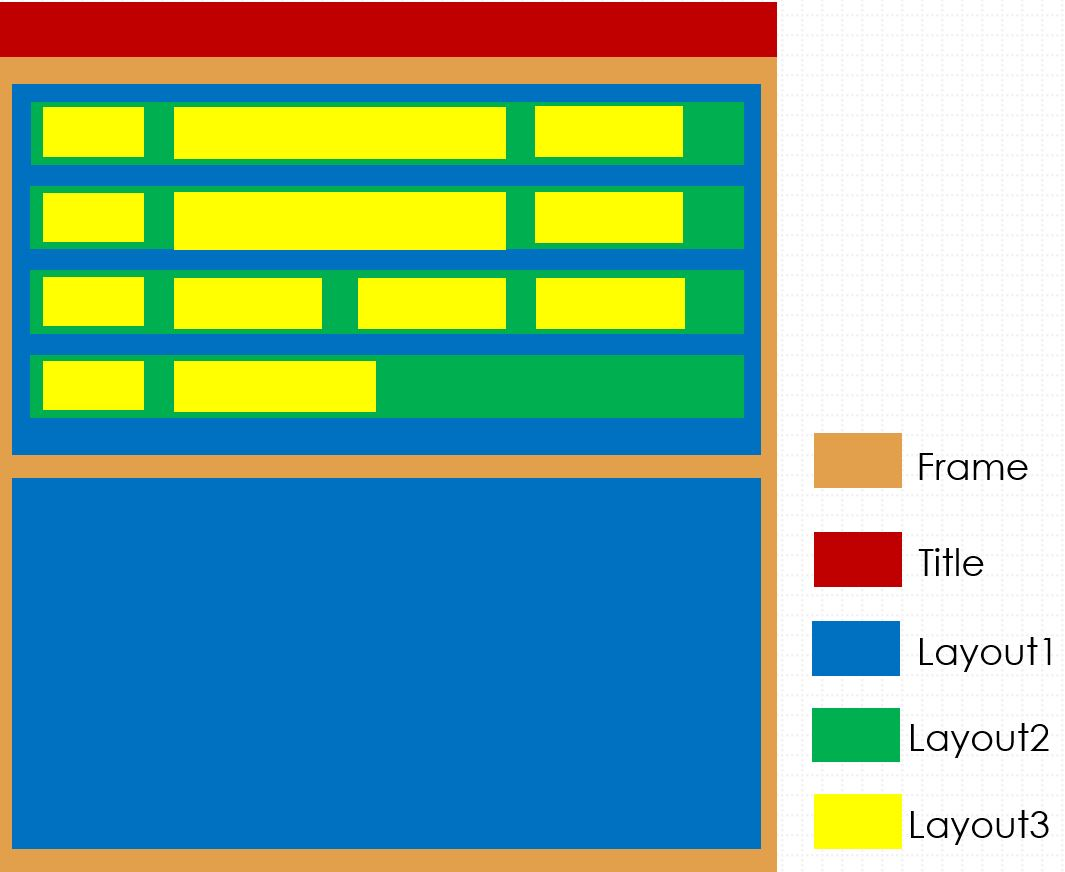
\includegraphics[width=7cm,height=5cm]{GUI设计}
  \caption{GUI设计框图}
\end{figure}

\column{7cm}
\begin{figure}
  \centering
  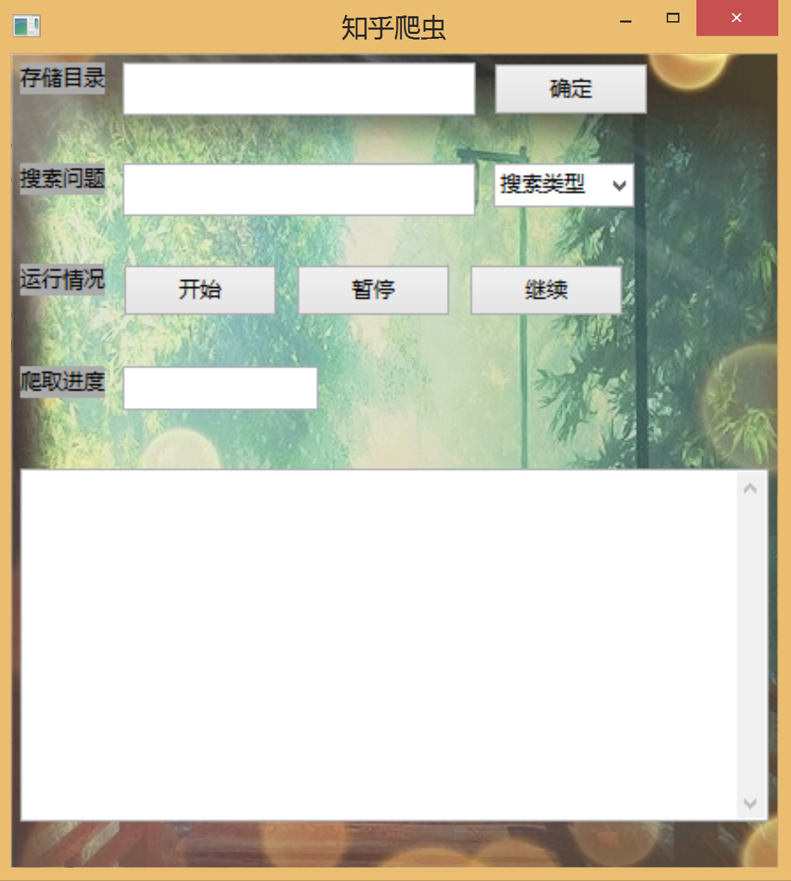
\includegraphics[width=6cm,height=5.5cm]{GUI界面}
  \caption{GUI界面}
\end{figure}
\end{columns}
\end{frame}

\begin{frame}{主程序流程}
\begin{figure}
  \centering
  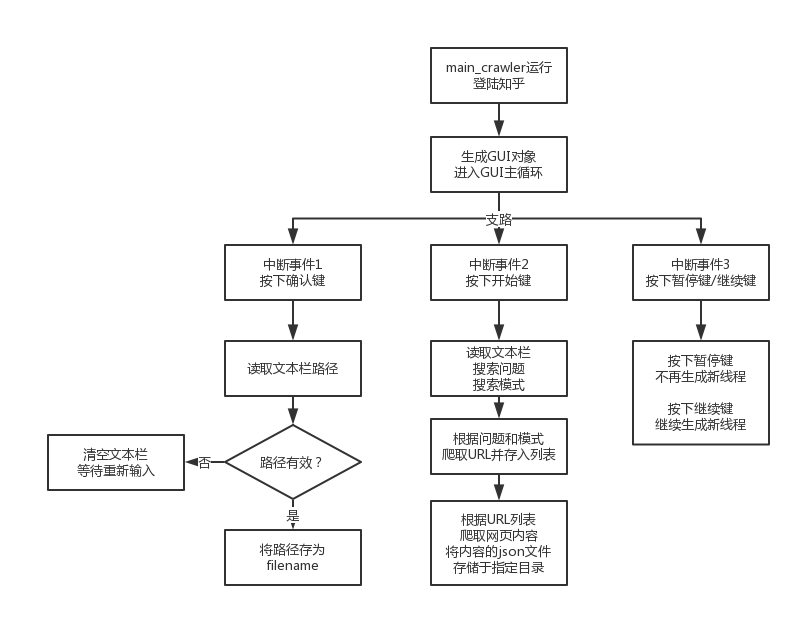
\includegraphics[width=9cm,height=6cm]{主程序流程图}
  \caption{主程序流程图}
\end{figure}
\end{frame}

\begin{frame}{多线程控制}
\begin{block}{Thread子类Crawler}\end{block}
\begin{figure}
  \centering
  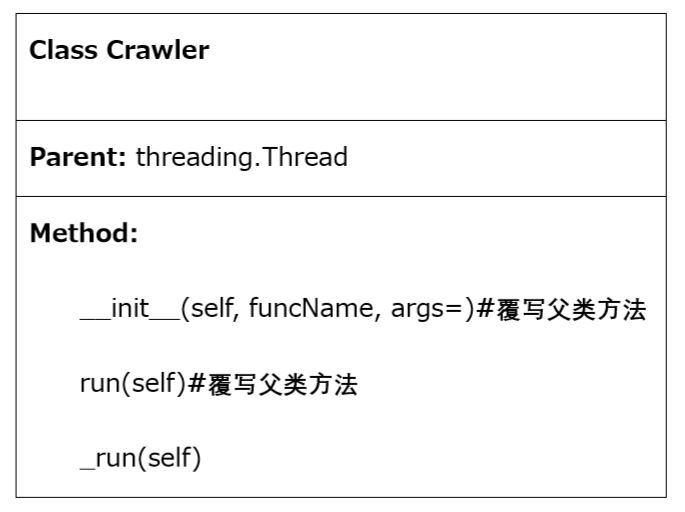
\includegraphics[width=8cm,height=5cm]{Crawl}
  \caption{Crawl}
\end{figure}
\end{frame}

\begin{frame}{多线程控制}
\begin{figure}
  \centering
  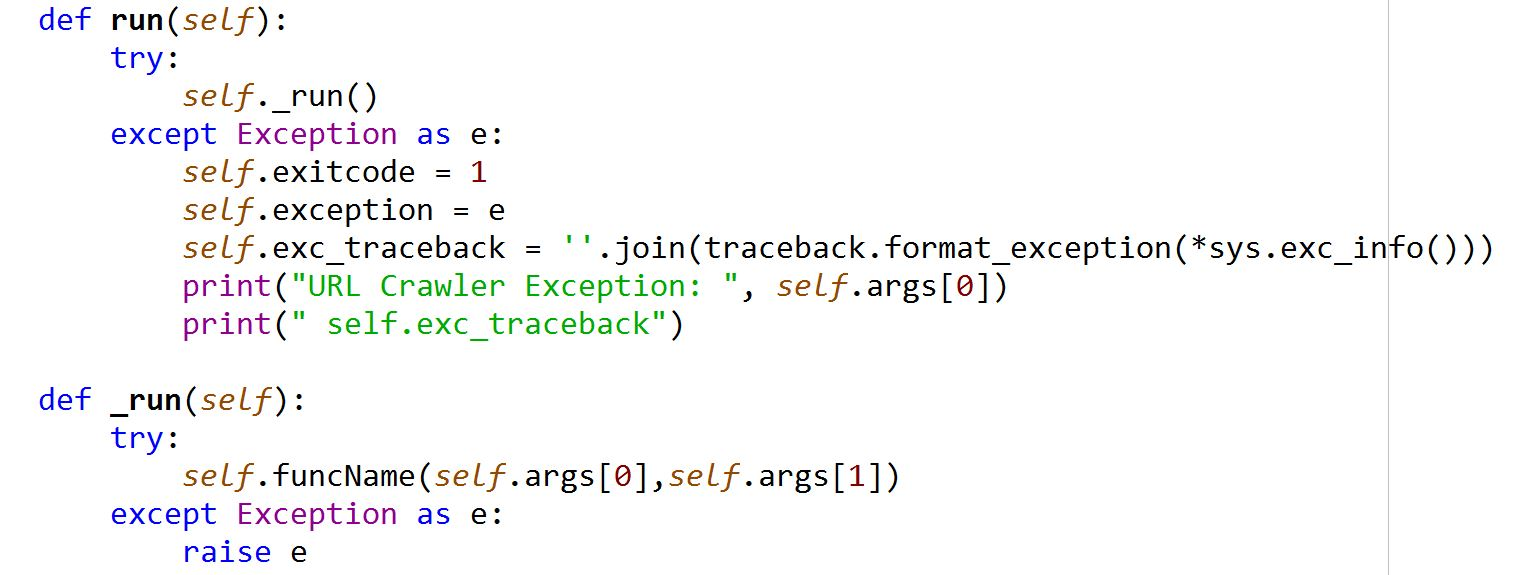
\includegraphics[width=13cm,height=5.5cm]{覆写run方法}
  \caption{覆写run方法}
\end{figure}
\end{frame}

\subsection{爬虫运行模块}
\begin{frame}{爬虫运行模块}
本模块主要实现了爬虫的基本运行,分为两个主要部分:
\begin{itemize}
  \item 知乎登陆
  \item 建立问题URL库
  \begin{itemize}
    \item 针对具体问题(Question)搜索知乎的“综合”模块
    \item 针对具体话题(Topic)搜索知乎的“话题”模块
  \end{itemize}
\end{itemize}
其中对问题(Question)的爬取采用PhantomJS库来实现动态加载,对话题(Topic)的爬取采用模拟翻页来实现动态加载。
\end{frame}

\begin{frame}{爬虫运行框图}
\begin{figure}
  \centering
  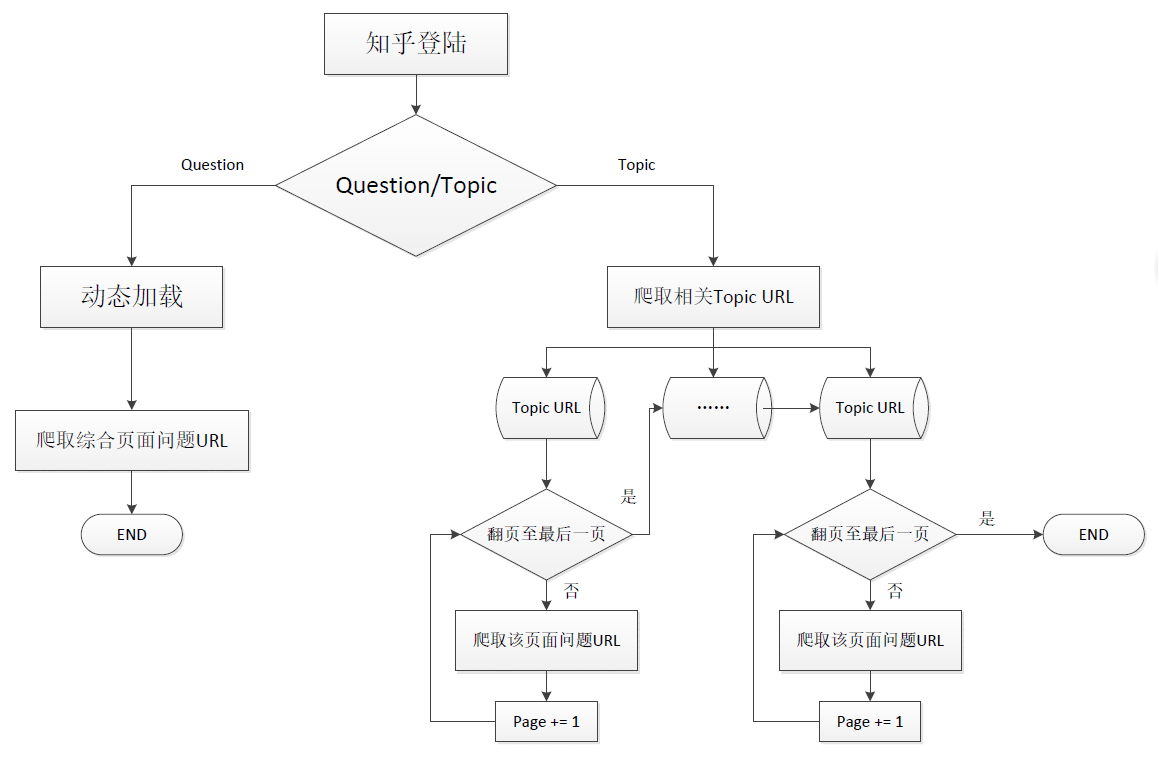
\includegraphics[width=9cm,height=6cm]{爬虫运行框图}
  \caption{爬虫运行框图}
\end{figure}
\end{frame}

\begin{frame}{知乎登陆}
\begin{block}{使用手机的代理(User-Agent)来模拟登陆}\end{block}
\begin{figure}
  \centering
  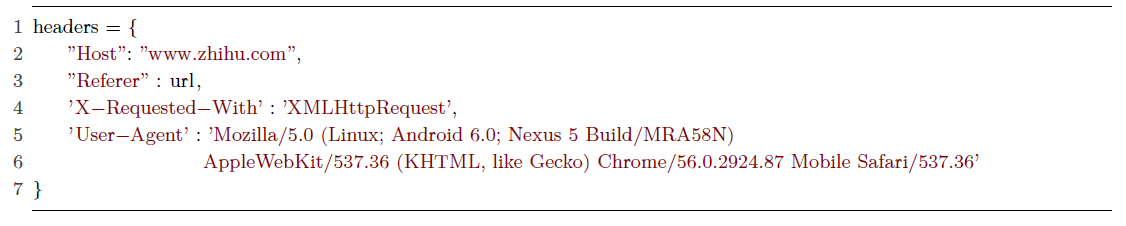
\includegraphics[width=15cm,height=3cm]{headers}
  \caption{headers头文件信息}
\end{figure}
\end{frame}

\begin{frame}{知乎登陆}
\begin{block}{采用验证码方式登陆,测试结果如下:}\end{block}
\begin{figure}
  \centering
  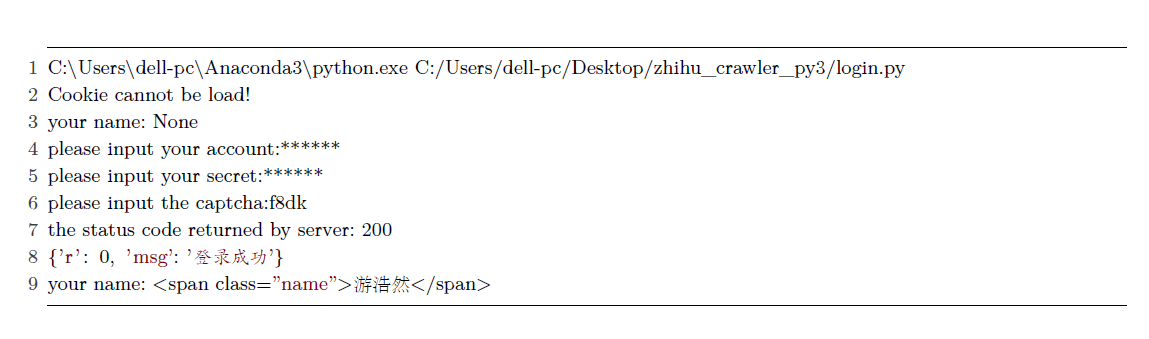
\includegraphics[width=13cm,height=4cm]{login}
  \caption{login}
\end{figure}
\end{frame}

\begin{frame}{网页下载和解析}
\begin{block}{网页下载函数即为下代码所示,使用requests库来抓取指定URL的内容:}\end{block}
\begin{figure}
  \centering
  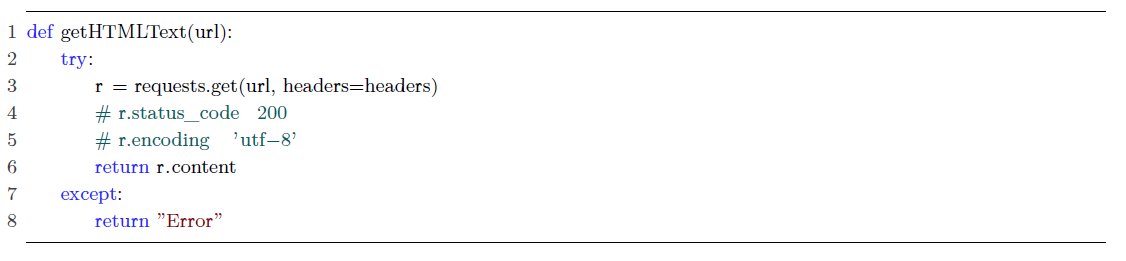
\includegraphics[width=13cm,height=3.5cm]{网页下载}
  \caption{网页下载}
\end{figure}
\end{frame}

\begin{frame}{网页下载和解析}
\begin{block}{网页解析函数即为下代码所示,使用BeautifulSoup库来抓取解析网页:}\end{block}
\begin{figure}
  \centering
  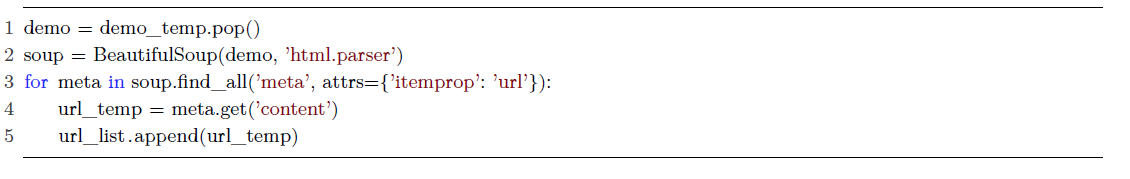
\includegraphics[width=13cm,height=2.5cm]{网页解析}
  \caption{网页解析}
\end{figure}
\end{frame}

\begin{frame}{URL爬取和管理}
\begin{itemize}
  \item 对知乎“综合”模块进行爬取
  \item 对知乎“话题”模块进行爬取
\end{itemize}
\begin{block}{存储为urllist[]列表格式供数据爬取模块调用}\end{block}
\end{frame}

\subsection{数据输出模块}
\begin{frame}{Question页面动态加载}
\begin{itemize}
  \item 问题的完整描述需要执行点击操作,使用selenium模拟
  \item 通过鼠标的下滑不断地动态加载,使用selenium模拟
\end{itemize}
\end{frame}

\begin{frame}{Question页面动态加载}
\begin{figure}
  \centering
  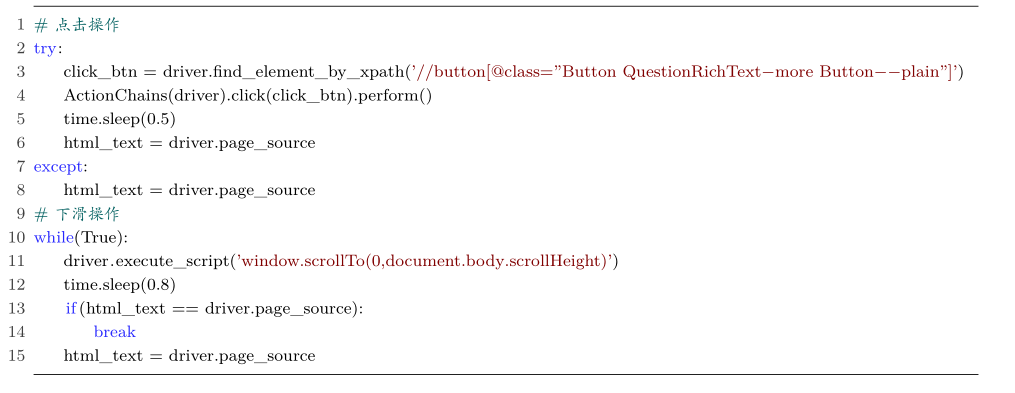
\includegraphics[width=13cm,height=5.5cm]{data}
  \caption{selenium模拟点击与下滑}
\end{figure}
\end{frame}

\begin{frame}{Question数据存储}
\begin{block}{效果展示}\end{block}
\begin{figure}
  \centering
  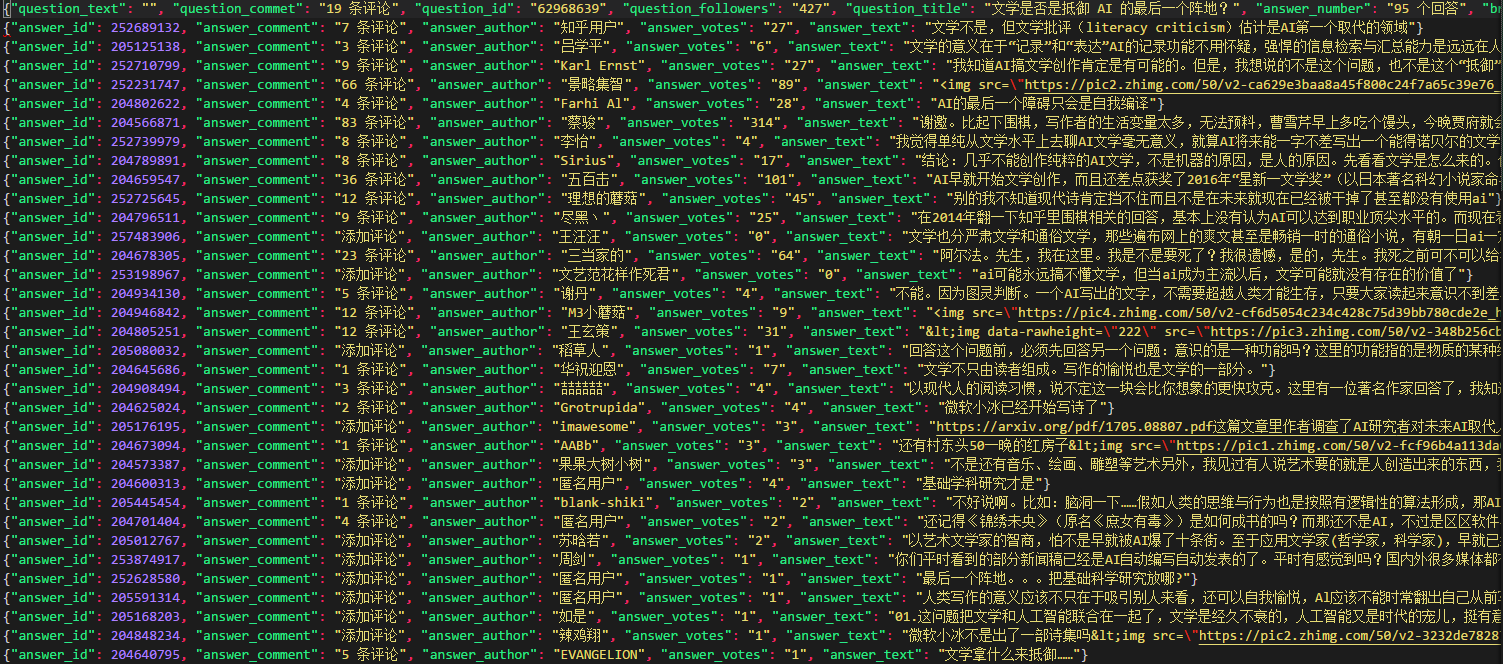
\includegraphics[width=12cm,height=5cm]{json}
  \caption{json效果展示}
\end{figure}
\end{frame}

\begin{frame}{Question数据存储}
\begin{figure}
  \centering
  
\includegraphics[width=12cm,height=2cm]{question}
  \caption{json效果展示}
\end{figure}
\begin{figure}
  \centering
  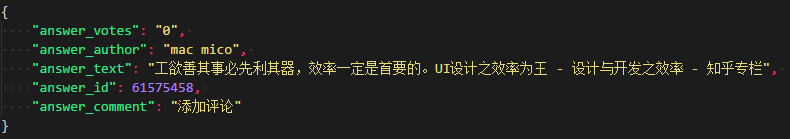
\includegraphics[width=12cm,height=2cm]{answer}
  \caption{json效果展示}
\end{figure}
\end{frame}
\section{Experiment}

\begin{frame}
\begin{itemize}[<+-| alert@+>]
\item Thank You.
\end{itemize}
\end{frame}

\end{document}
